%!TEX root = ../document.tex
\chapter{Raspberry}
\label{ch:Raspberry}
\section{Grundlegendes}
\label{sc:RPIGrund}
Das Raspberry Pi 3 Model B ist ein in Großbritannien gebauter Ein-Platinen Computer. Dieser Mini-PC ist in der Lage grundlegende Tätigkeiten eines Desktop-Computers zu realisieren. Er verfügt über die Möglichkeit diverse Betriebssysteme und eigene Programme zu schreiben und anzuwenden. Das Pi 3 besitzt jedoch wie seine Vorgänger keine Festplatte, es wird stattdessen eine Micro-SD-Karte oder ein USB-Stick verwendet. Der Raspberry Pi besitzt außerdem die Möglichkeit durch verschiedene Schnittstellen elektronische Schaltungen und Projekte zu kreieren und diese zu steuern. Durch die fest verbauten Anschlüsse ist es zudem möglich verschiedene Aus- und Eingabegeräte mit dem Raspberry Pi 3 zu verbinden. In der folgendem Bild ist ein physikalischer Aufbau zu sehen.
	\begin{figure}[H]
		\centering
		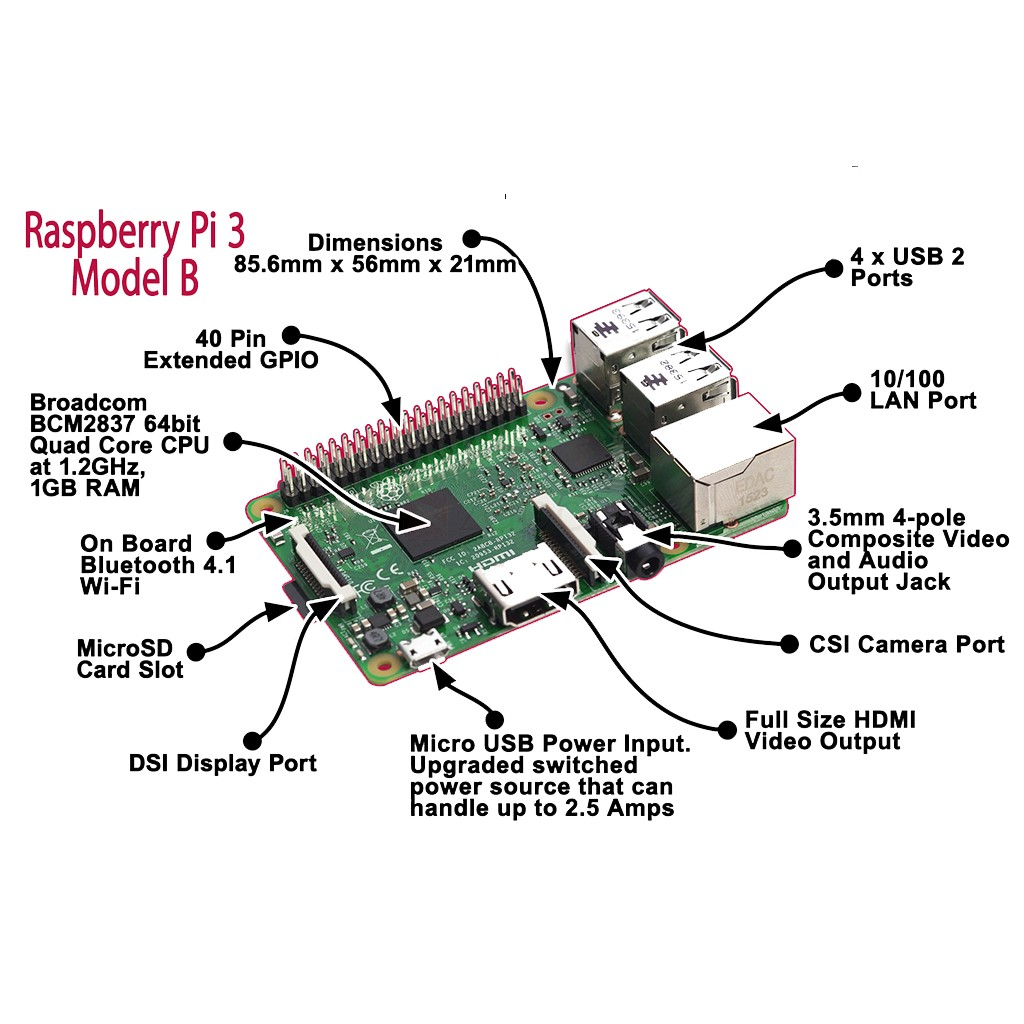
\includegraphics[width=1.0\textwidth]{images/raspberry_aufbau/raspberry_pi_3_model_b.jpg}
        \label{fig:raspberry_aufbau}
		\caption{Raspberry Pi 3 Model B}
	\end{figure}
Das Raspberry 3 Model B enthält einen 4-Kern-CPU mit 1,2 GHz von und 64-Bit sowie 1 GB RAM. Es beinhaltet ein integriertes drahtloses Netzwerk, Bluetooth, Ethernet 100 mbit/s und vier verbaute USB-Buchsen. Es verfügt außerdem über 40 GPIO-Pins, DSI Display Port, Full Size HDMI Video Output und ein CSI Camera Port, sowie einen 3.5mm 4-pole Composite Video and Audio Output Jack. Als Stromquelle ist ein standardmäßiges Micro USB-Netzteil mit 5V und 2000 mA vorgesehen. Weitere Bauteilbezeichnungen und Hardwaredaten sind in Abbildung \ref{fig:raspberry_aufbau} zu sehen.

\subsection{SD Karte}
    	\begin{figure}[H]
		\centering
		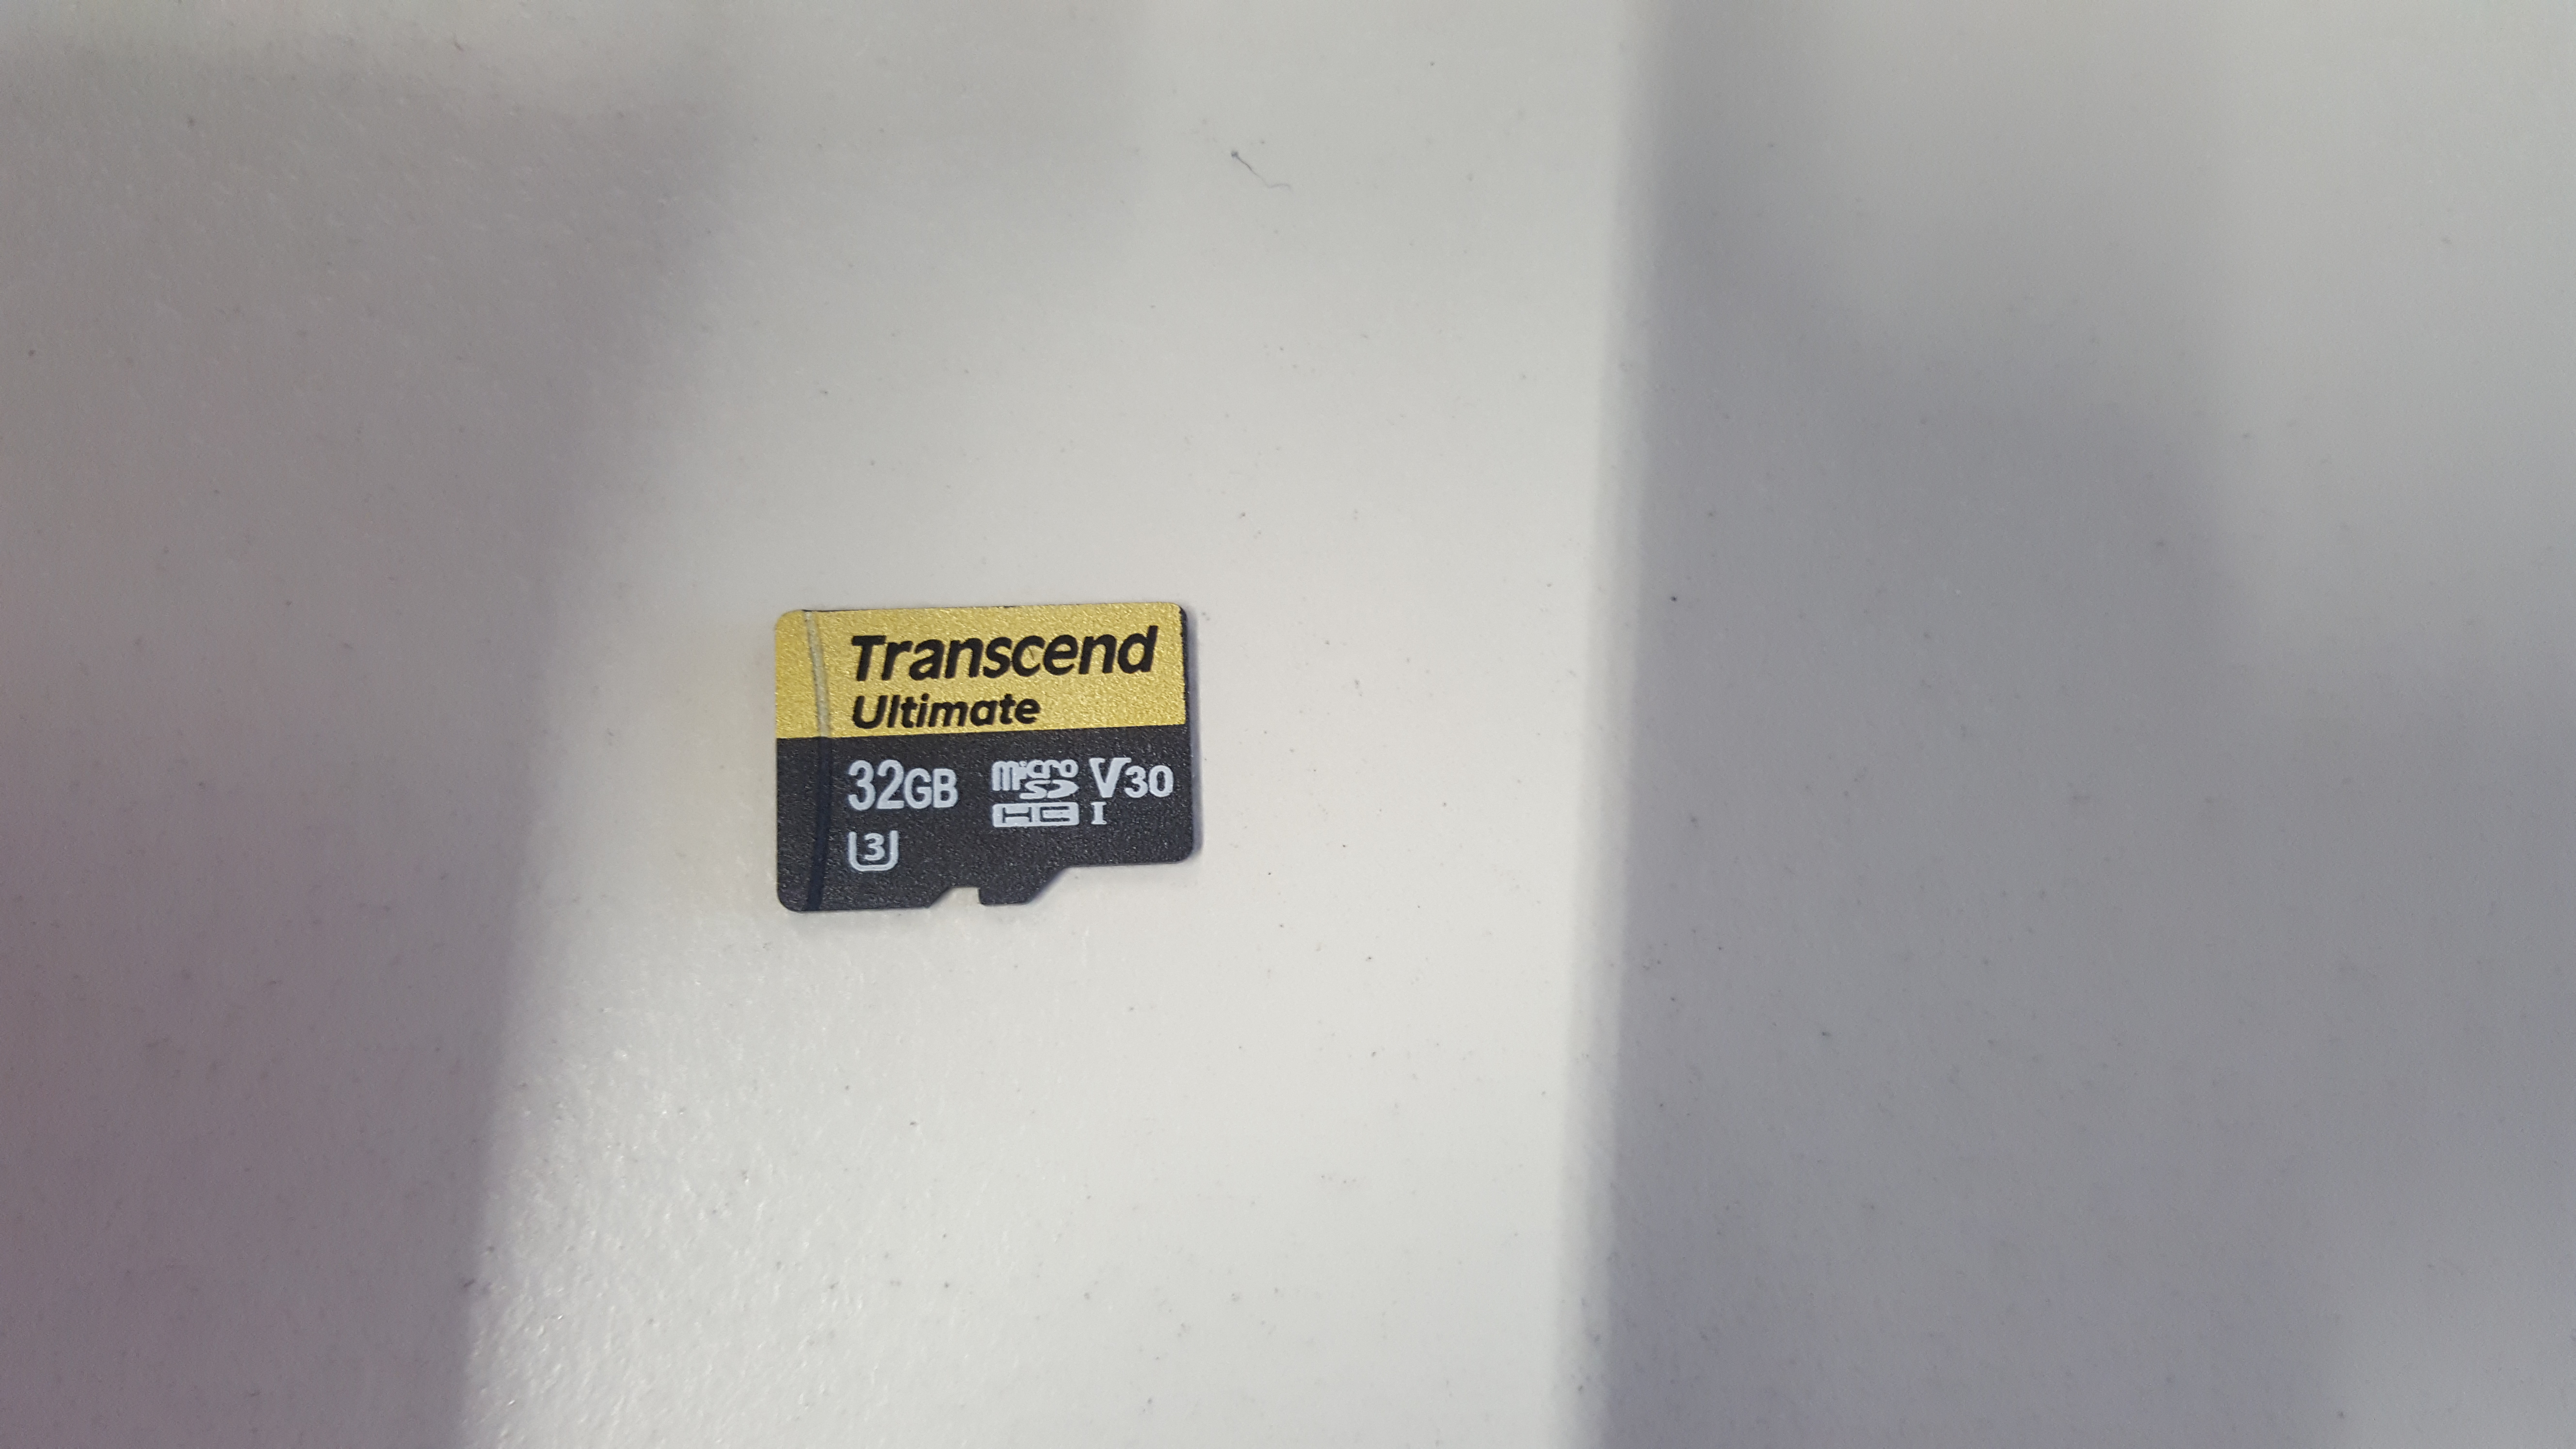
\includegraphics[width=1.0\textwidth]{images/raspberry_aufbau/MikroSdCard.jpg}
		\caption{Micro-SD Karte}
	\end{figure}
Die Micro-SD Karte dient initial als Festplattespeicher, welche das Betriebssystem enthält. Das Raspberry ist Werksseitig so eingestellt, dass dieses immer von der SD Karte bootet. Ist keine SD Karte eingelegt, kann kein Bootvorgang stattfinden. Grund dafür ist, dass  auf den BCM 2835, 6 und 7 Chip sich ein 32kb Speicher befindet der das Booten ermöglicht. Dieser sucht bei jedem Bootvorgang die Datei "bootecode.bin" auf der SD-Karte. Im Laufe des Projekts "Security Workbench" wurde entschieden, dass die SD Karte weggelassen wird, da der Zugang wegen dem Touchbildschirm und dem damit verbundenen Gehäuse blockiert wird. Zudem hat die Erfahrung gezeigt, dass SD Karten einen hohen Verschleiß bei signifikanten Lese und Schreibarbeiten aufweist. Abhilfe schafft ein bootfähiger USB-Stick. Dazu wird im kommenden Kapitel genauer erläutert.
 
\subsection{USB Stick}
    	\begin{figure}[H]
		\centering
		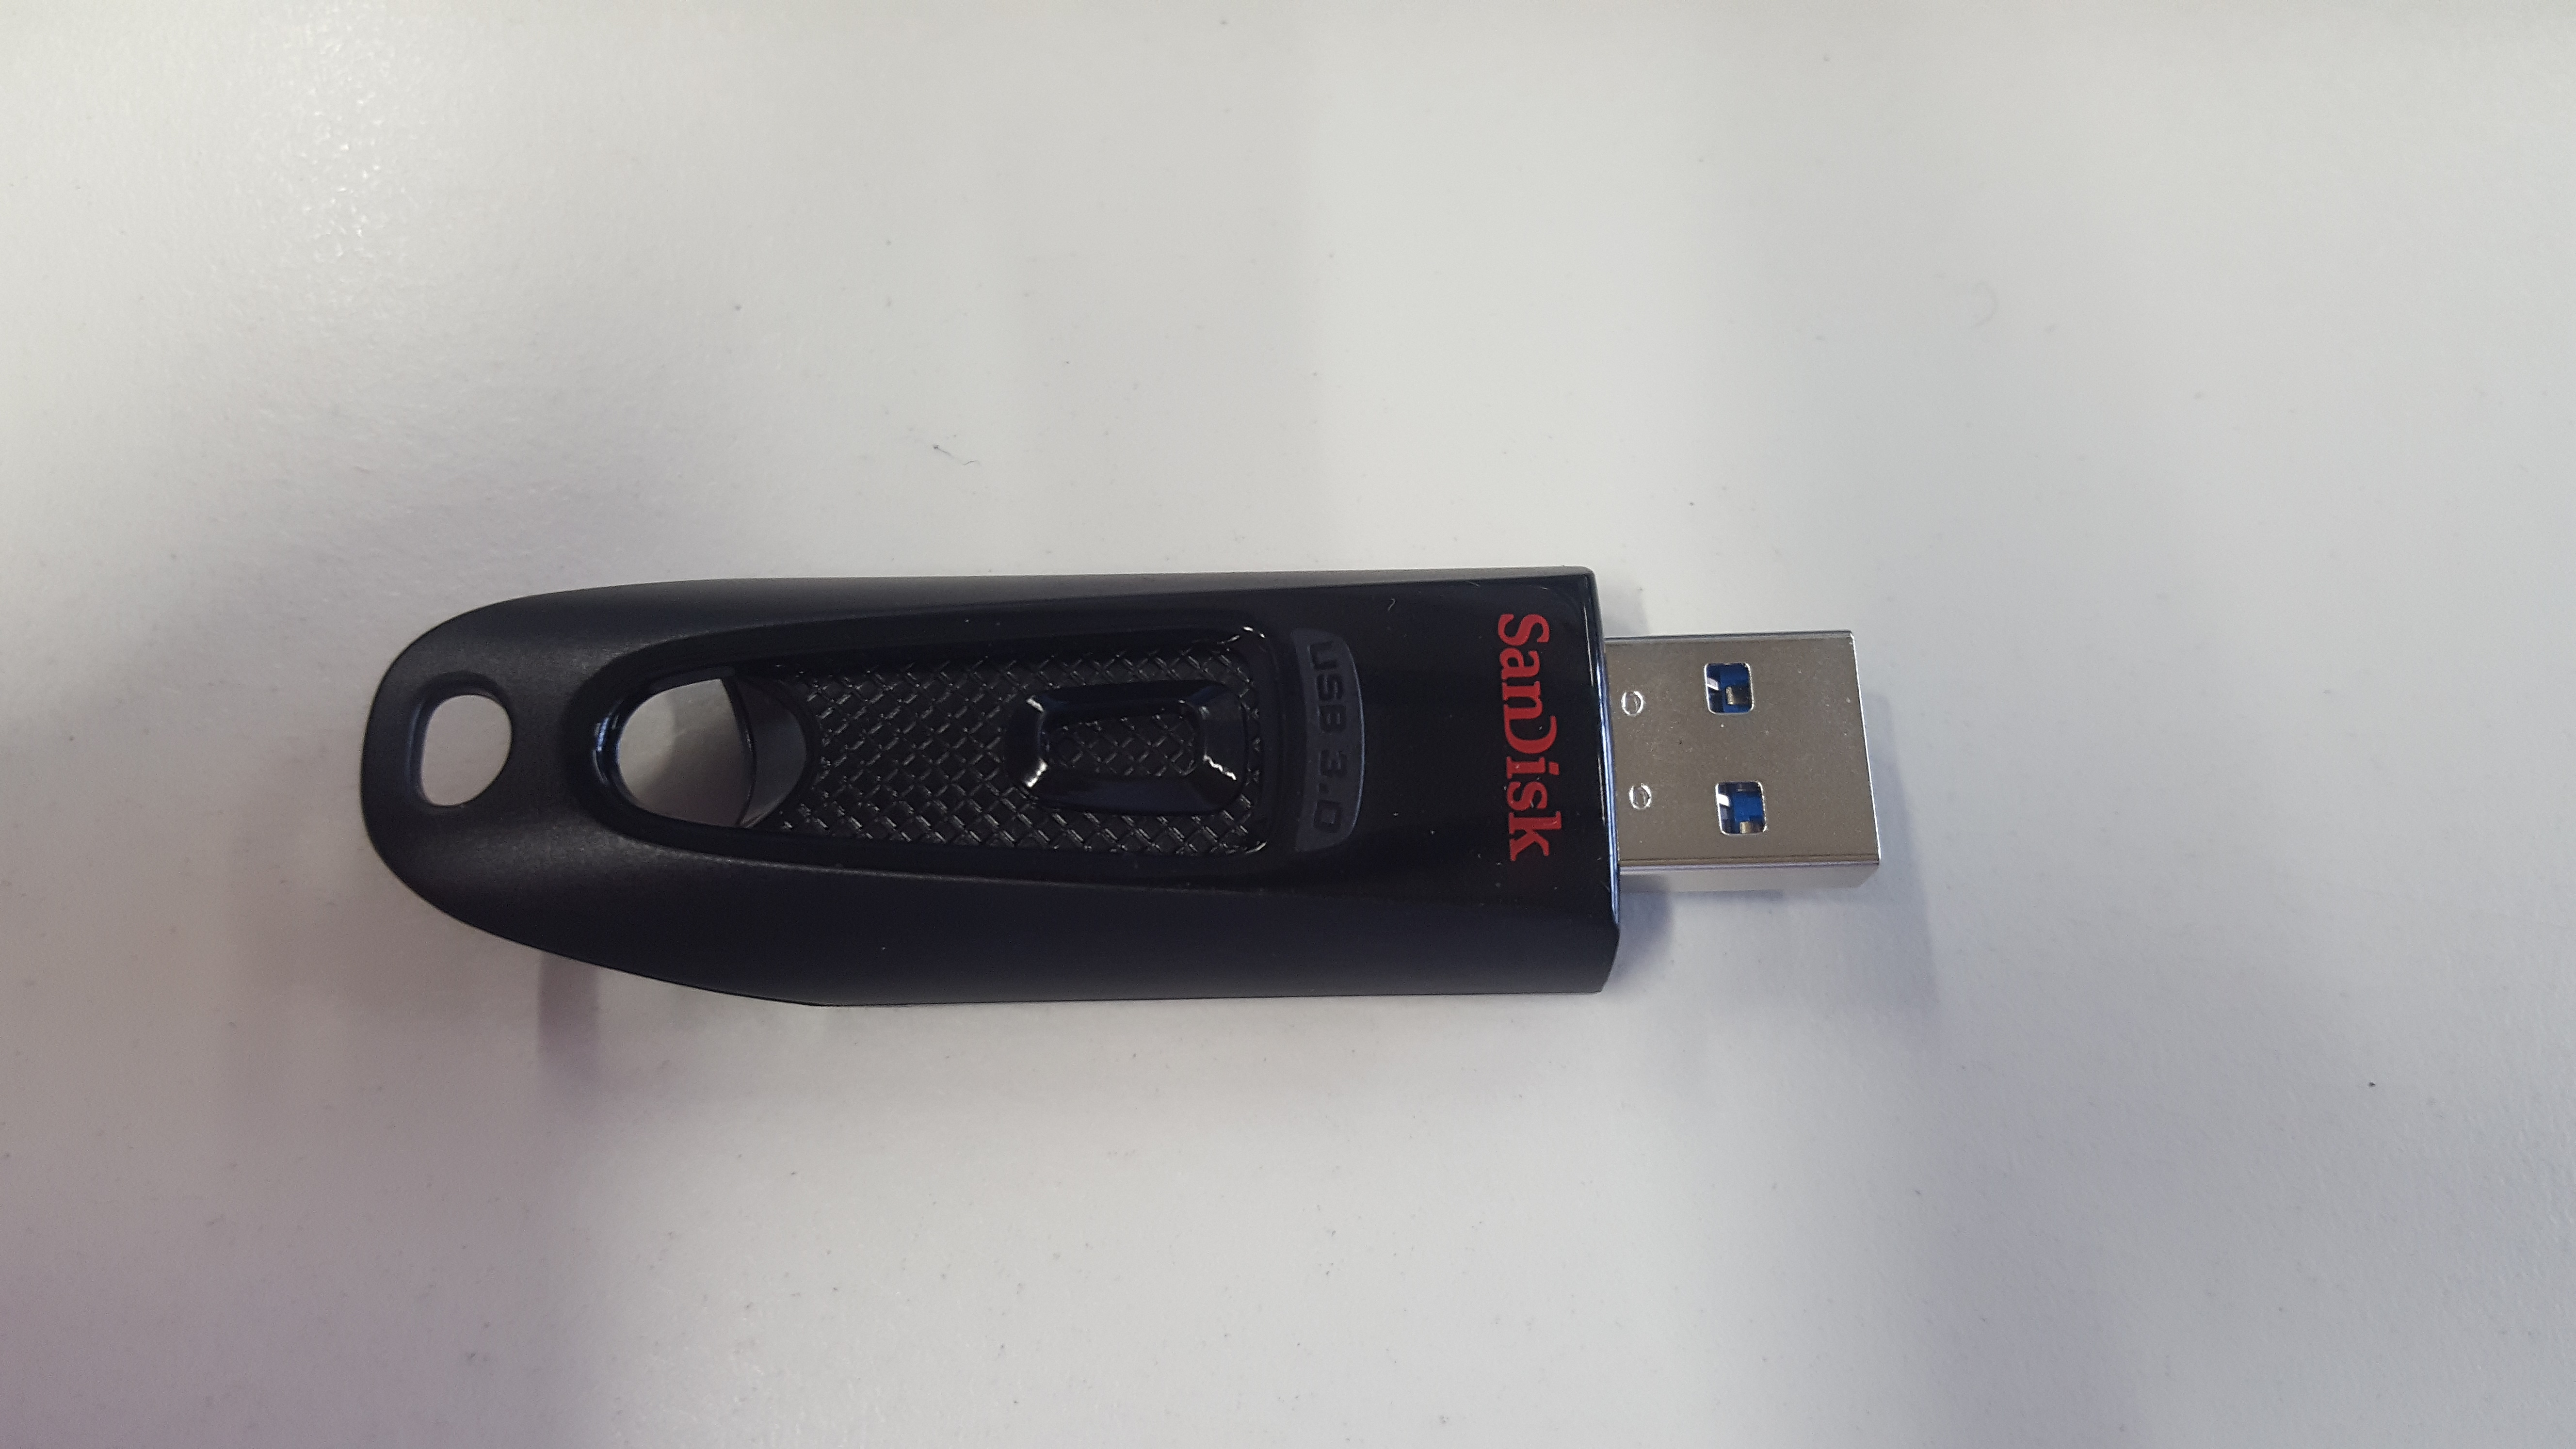
\includegraphics[width=1.0\textwidth]{images/raspberry_aufbau/UsbStick.jpg}
		\caption{USB Stick}
	\end{figure}  
Ab dem Raspberry Pi 3 Model b ist es möglich einen Bootfähigen USB-Stick zu konfigurieren. Die Entwickler der Raspberry Pi Foundation entwickelten extra dafür einen neuen Bootloader. Somit ist man nun in der Lage von verschiedenen Medien zu booten. Dadurch ist eine komfortable Lösung geschaffen, welches ein einfaches und schnelles wechseln des Betriebssystems ermöglicht. Das Raspberry Pi besitzt, statt eines BIOS, eine Datei namens "config.txt". Dort werden verschiedene Parameter übergeben, welche das Raspberry Pi zum booten benötigt. Diese neue Funktion des Bootloaders wurde in diesem Projekt zunutze gemacht. Deshalb wurde in die Datei "config.txt" die Zeile "program\_usb\_boot\_mode = 1" hinzufügt und anschließend das Pi heruntergefahren. Ist daraufhin ein USB-Stick mit z.B. einer Linux Partitionen mit dem Raspberry verbunden, kann die SD Karte entfernt werden und neugestartet werden. Nach kurzer Zeit ist zu sehen, dass der Boot via USB-Stick erfolgreich war. Dieser Zustand ist nun auf Dauer gültig und muss nicht am selben Gerät wiederholt werden. Es ist trotzdem zu beachten, dass bei jedem Raspberry eine Initiale Einrichtung über eine SD-Karte erfolgen muss.

\subsection{W-Lan Antenne}
    	\begin{figure}[H]
		\centering
		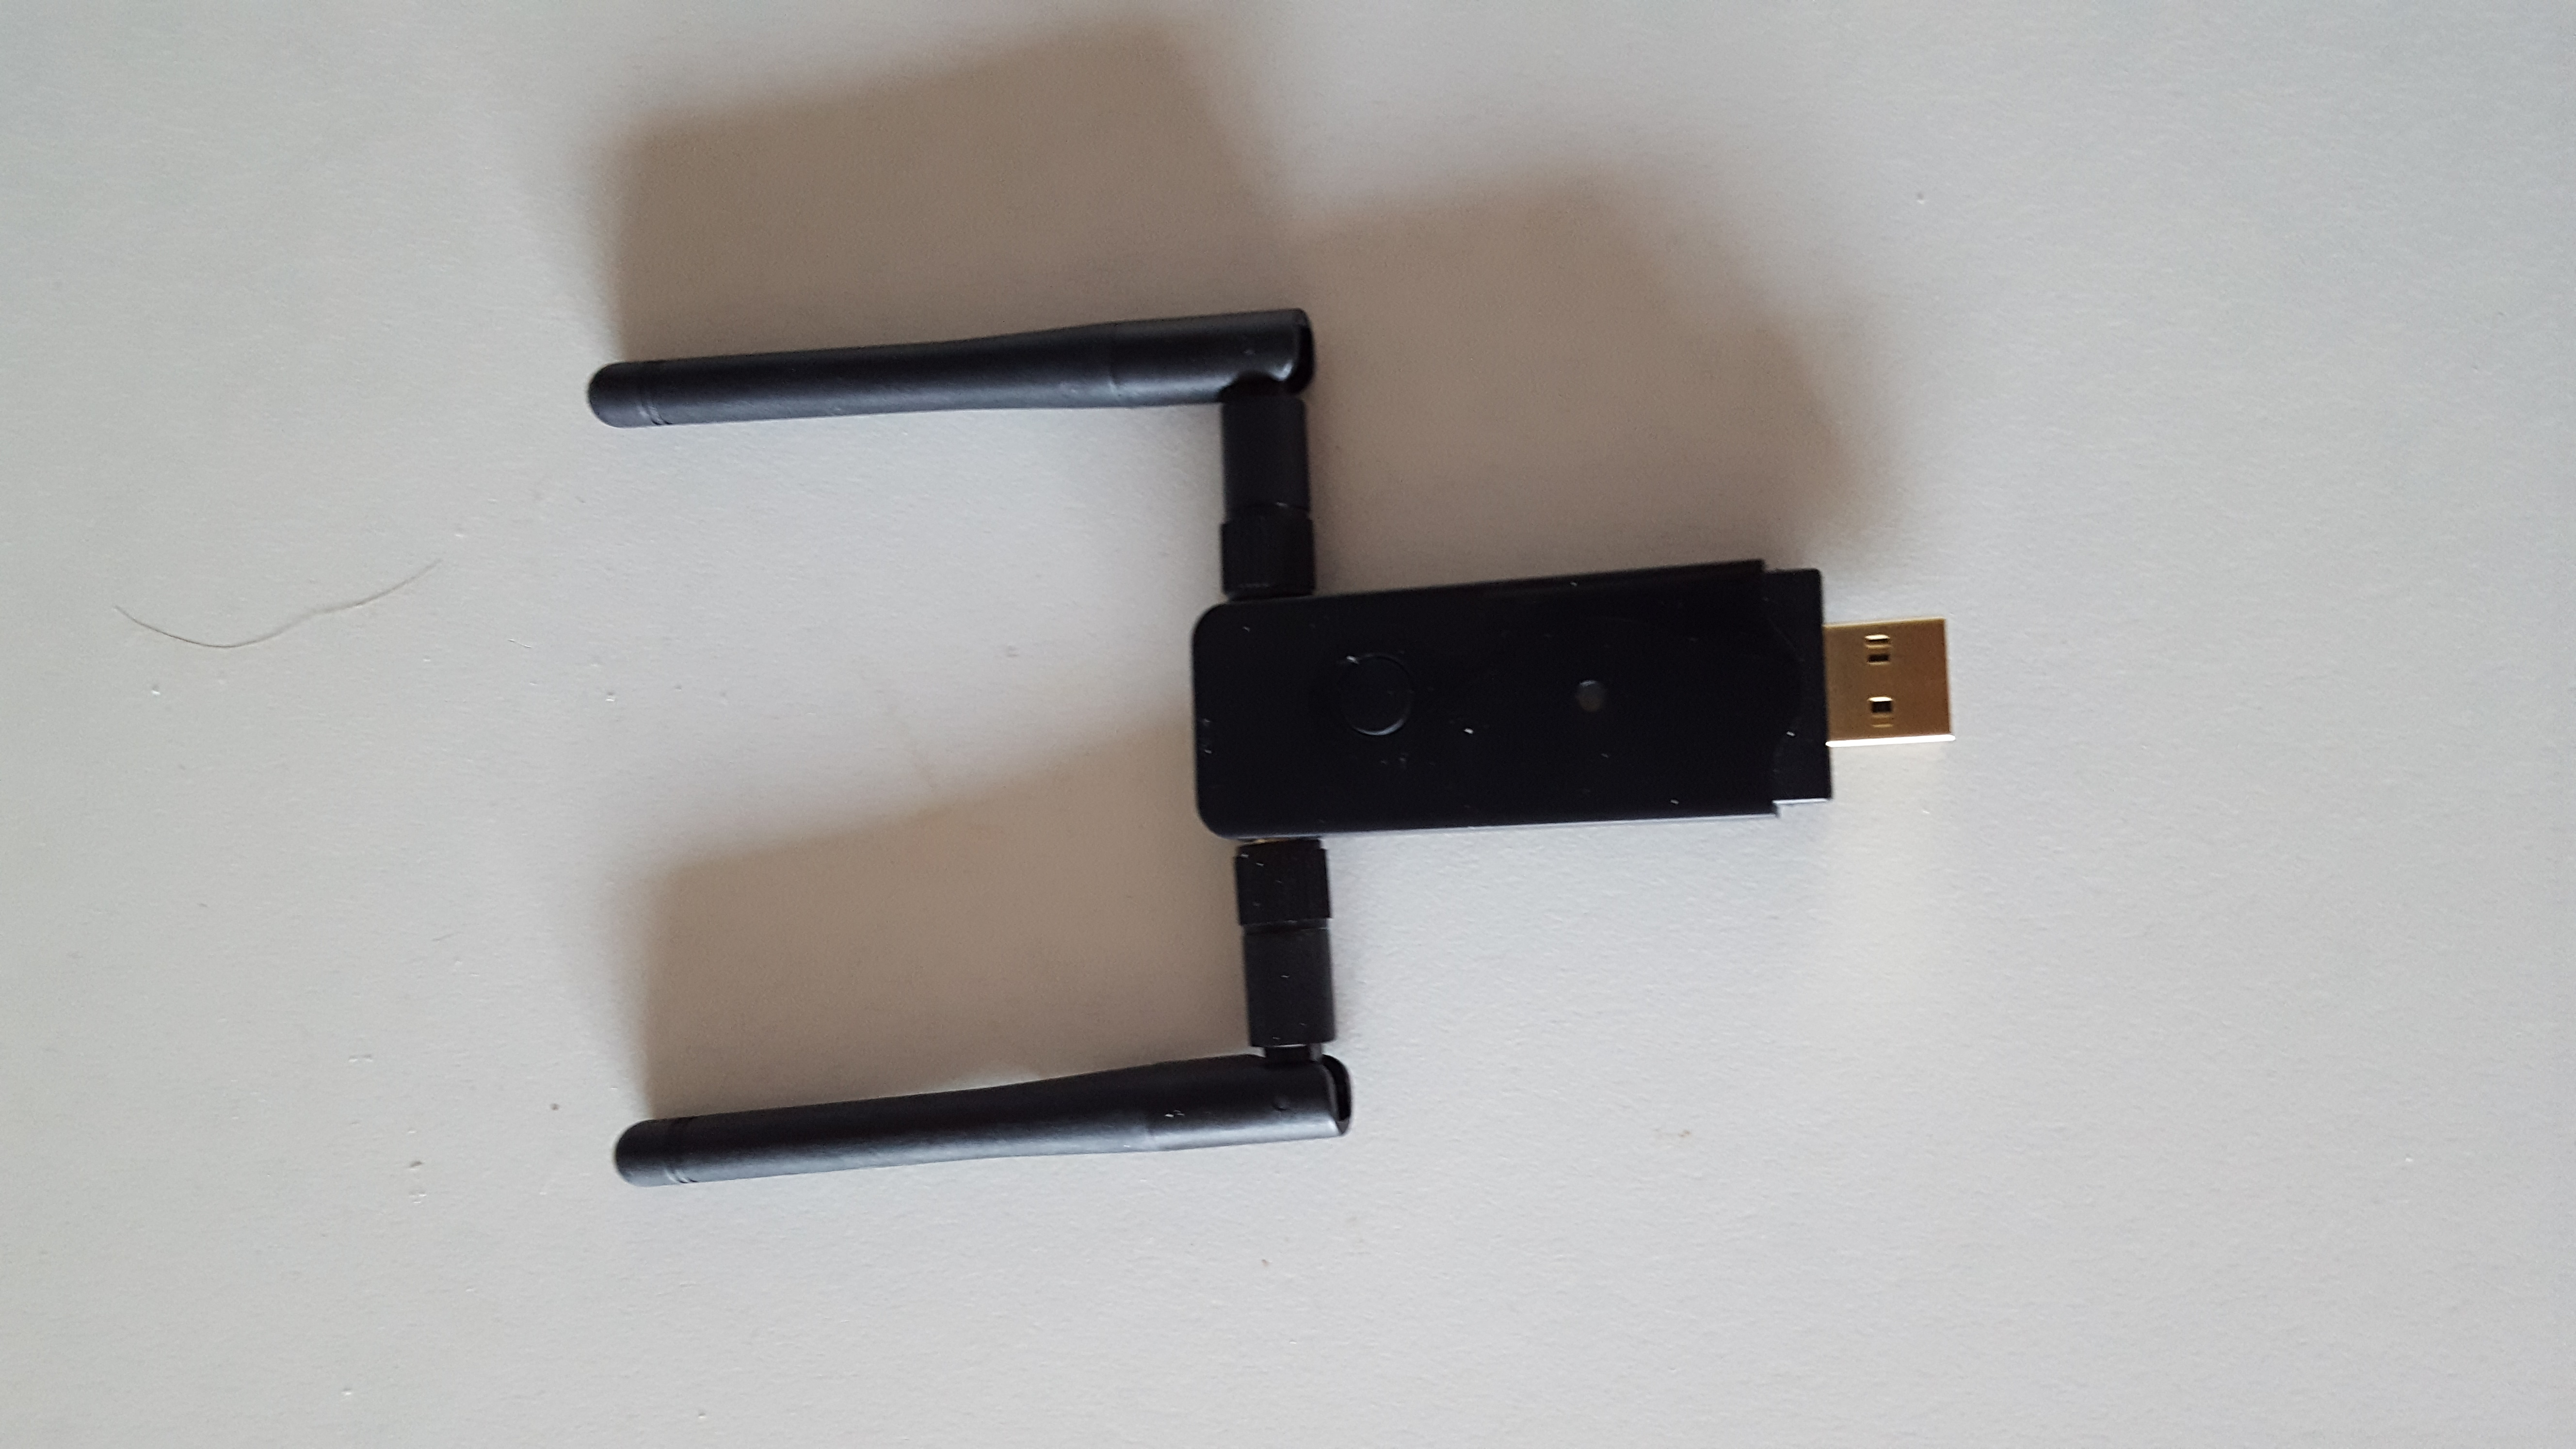
\includegraphics[width=0.95\textwidth]{images/raspberry_aufbau/WlanAntenne.jpg}
        \label{fig:wlan}
		\caption{WLAN-Antenne}
	\end{figure}
Für den, von Raspberry Foundation, zur Verfügung gestellten Access-Point, war es leider nicht möglich auf das schon integrierte WLAN-Modul zu setzten, da es den Standard für WPA2-Enterprise Access-Points nicht unterstützte. Um diese Problematik zu beheben, wurde ein USB-WLAN-Stick verwendet, der diesen Standard unterstützt (siehe Abbildung\ref{fig:wlan}).
\subsection{Switch}
    	\begin{figure}[H]
		\centering
		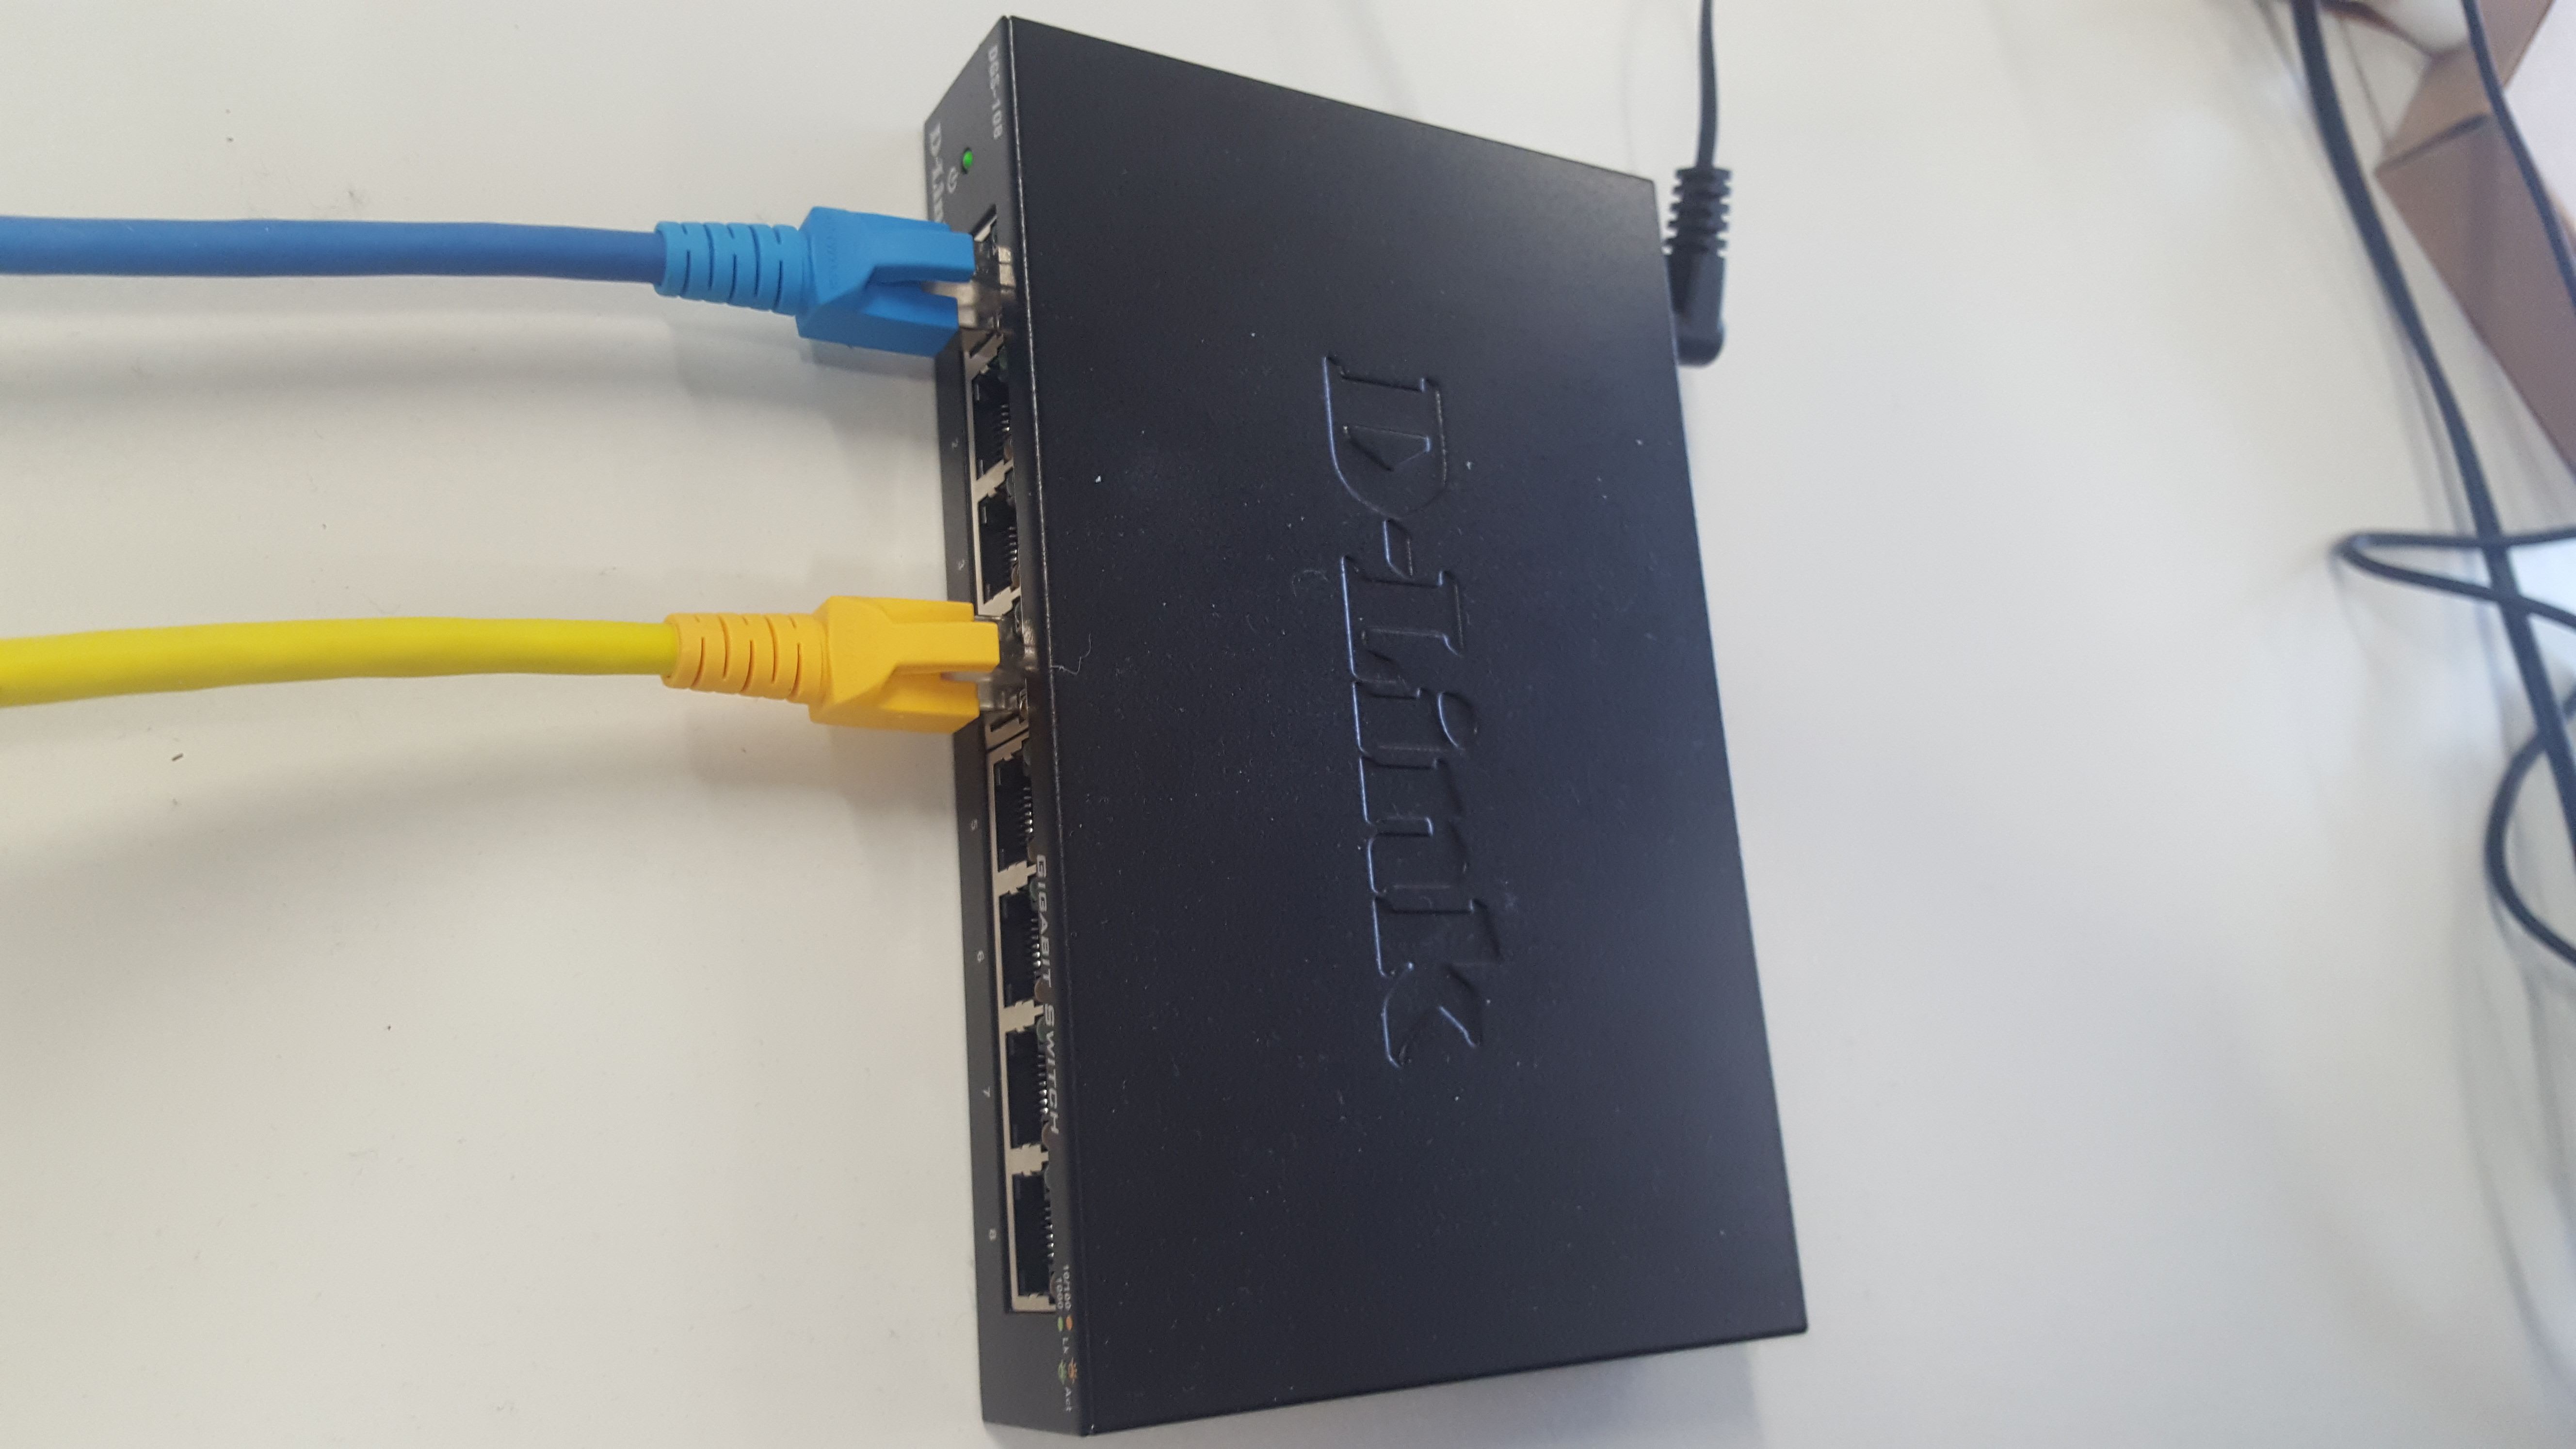
\includegraphics[width=1.0\textwidth]{images/raspberry_aufbau/Switch.jpg}
        \label{fig:switch}
		\caption{Switch}
	\end{figure}
Um die drei Raspberries untereinander zu verbinden, kann man auf einen handelsüblichen L2-Switch, wie z.B. in Abbildung\ref{fig:switch} zu sehen, verwenden.

\subsection{Gesamtansicht}
    	\begin{figure}[H]
		\centering
		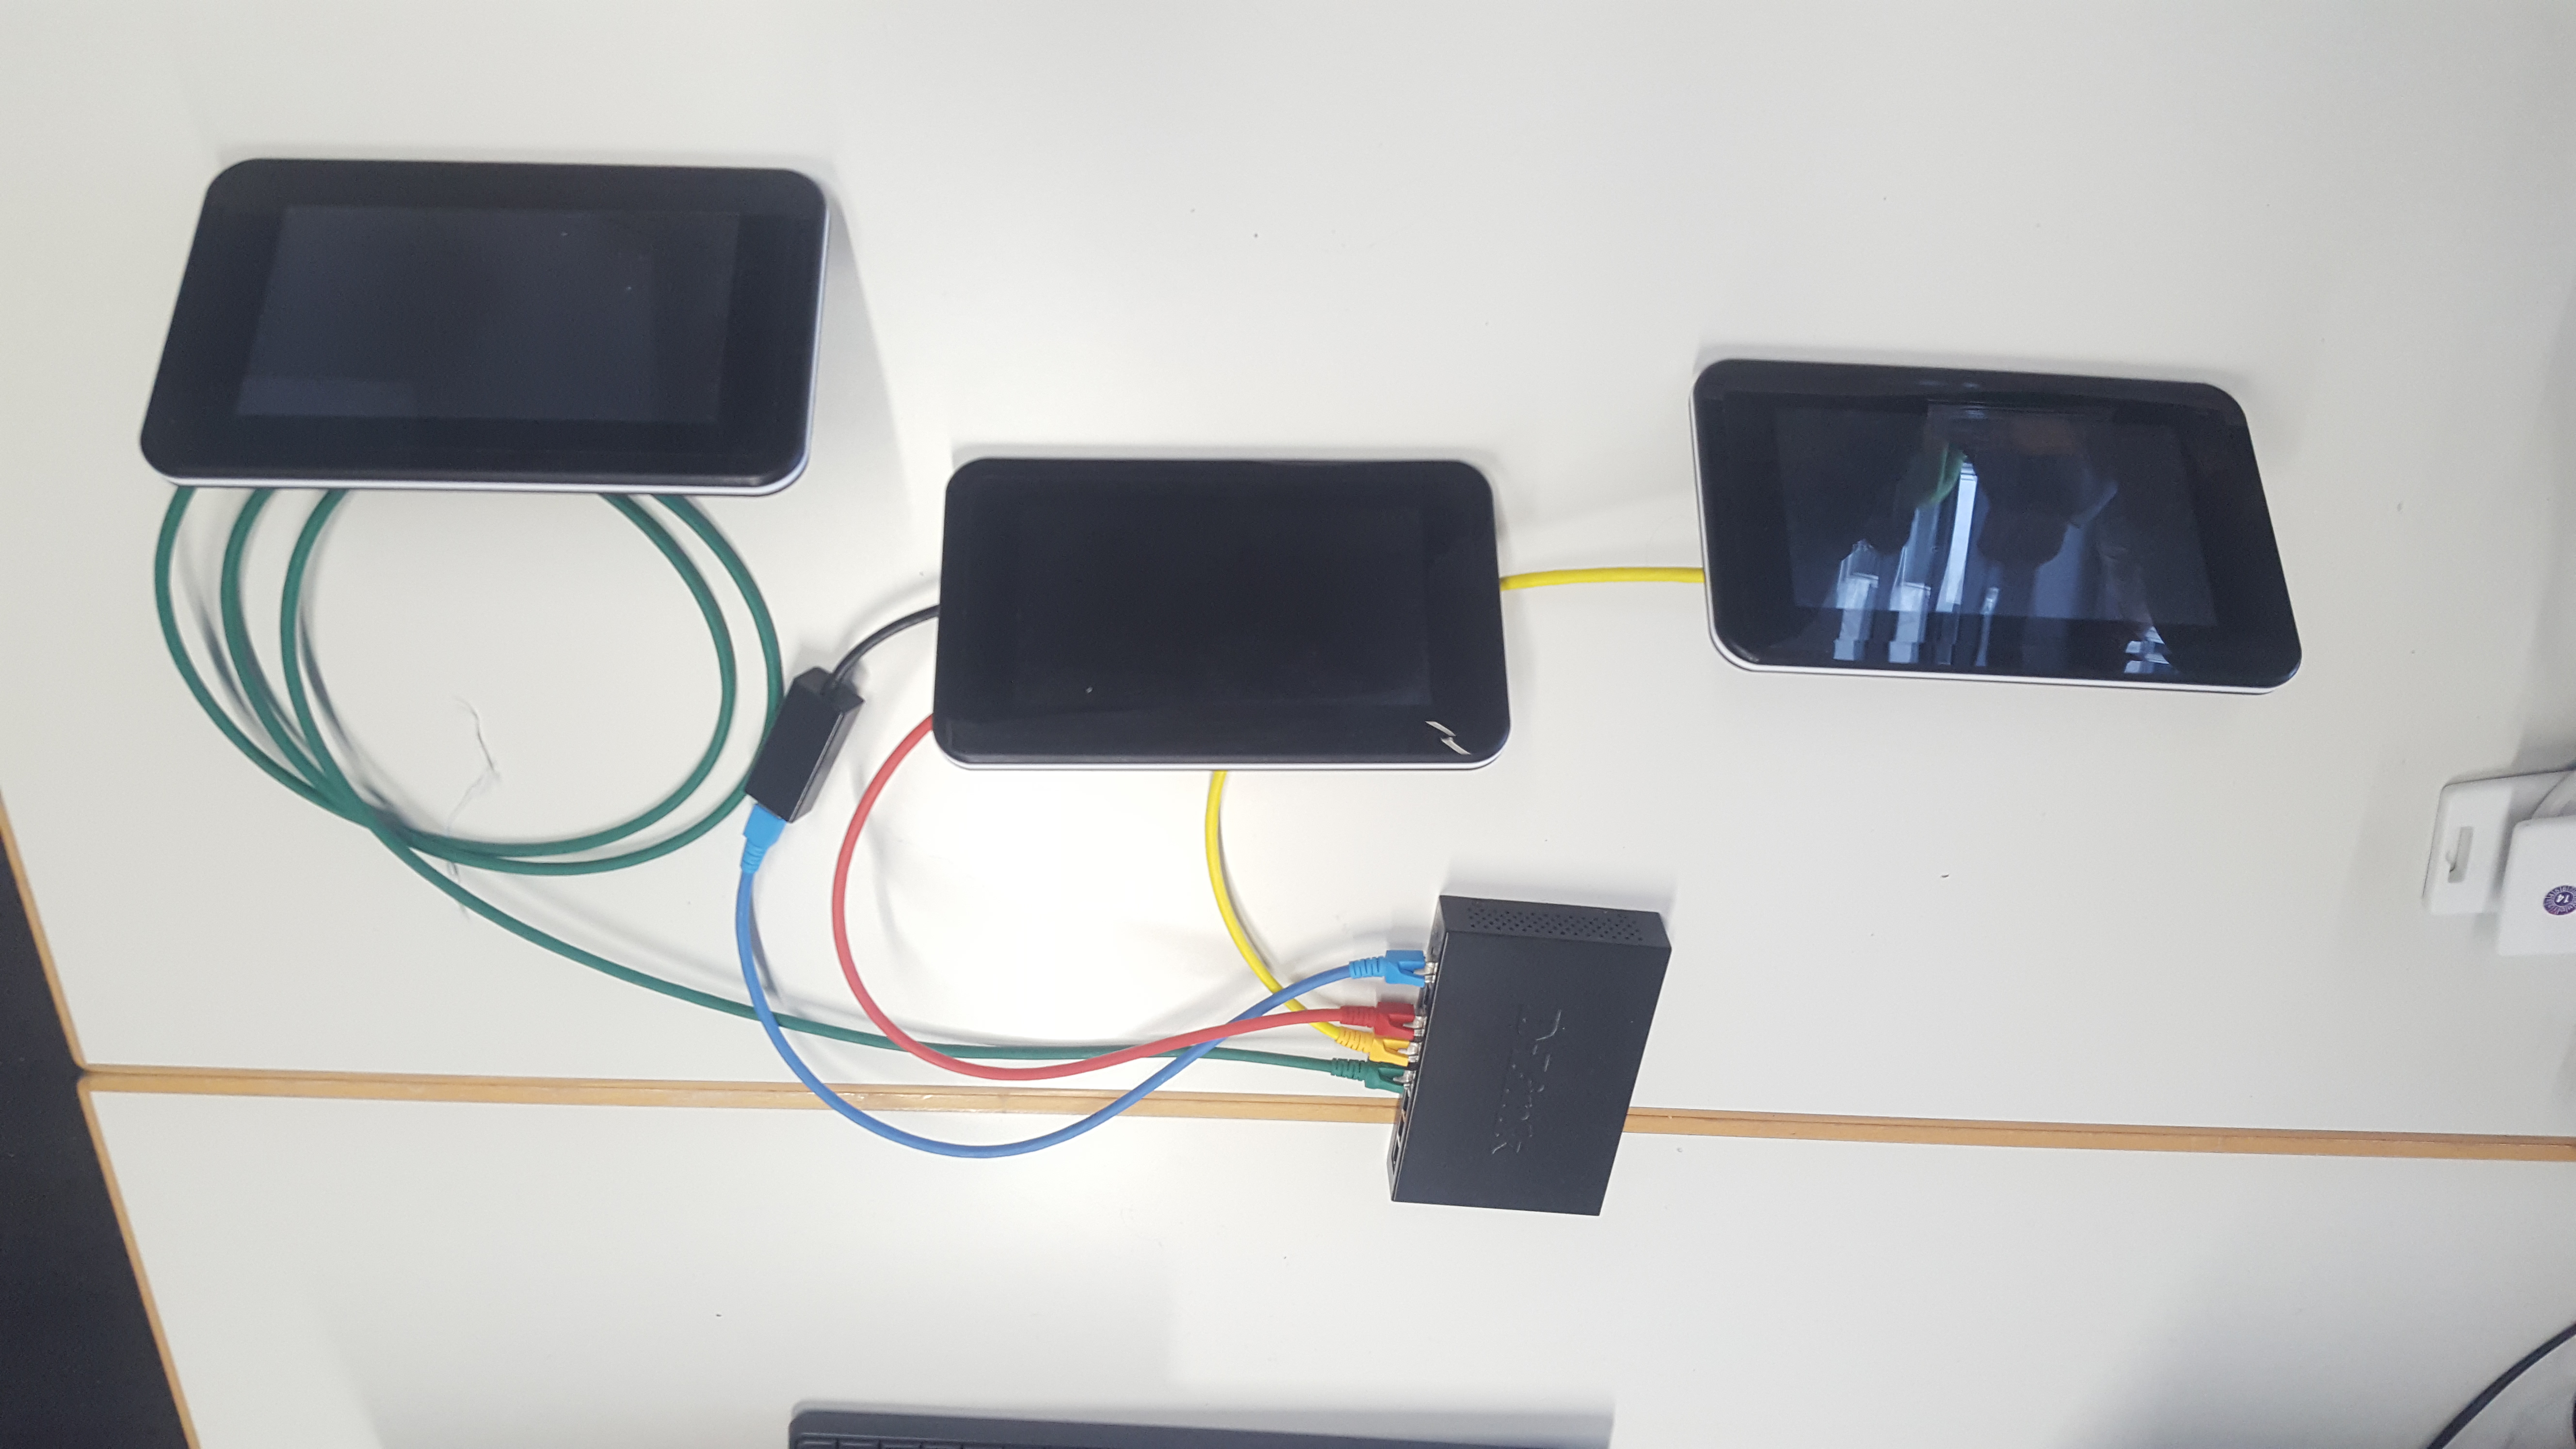
\includegraphics[angle=180, width=1.0\textwidth]{images/raspberry_aufbau/gesAns.jpg}
		\caption{Gesamtansicht der Workbench}
	\end{figure} %TODO schematischer Aufbau einfügen
Die Security-Workbench ist in drei unterschiedliche Komponenten aufgeteilt. Die beiden Raspberry Pi's, links und rechts auf dem Bild, sind so konfiguriert, dass sie Opfer oder Angreifer sein können. Das Raspberry dazwischen, dient als Server und WLAN-Schnittstelle. Alle Komponenten sind über einen Switch verbunden, welcher vom WAN abgetrennt ist, somit bleibt das Hochschulnetzwerk unberührt. Die Voraussetzungen für das Tutorial auf den Raspberry Pi's sind wie folgend:\\
\begin{enumerate}
	\item Alle drei Raspberry Pi's müssen entsprechend der Gesamtansicht, mittels Ethernetkabel, mit dem Switch verbunden werden.
    \item Beim Raspberry Pi, welcher als Server und Wlan-Schnittstelle dient, muss der Netzwerkadapter und die Wlan-Antenne zusätzlich angeschlossen werden.
    \item Alle benötigten Geräte an das Stromnetz anschließen. 
\end{enumerate}
Im folgenden Kapitel, Installationsanleitung für Raspberry, wird das Aufsetzen der Betriebssysteme auf die Raspberry Pi's genauer erläutert.